\pdfminorversion=4
\documentclass[aspectratio=169]{beamer}

\mode<presentation>
{
  \usetheme{default}
  \usecolortheme{default}
  \usefonttheme{default}
  \setbeamertemplate{navigation symbols}{}
  \setbeamertemplate{caption}[numbered]
  \setbeamertemplate{footline}[frame number]  % or "page number"
  \setbeamercolor{frametitle}{fg=white}
  \setbeamercolor{footline}{fg=black}
} 

\usepackage[english]{babel}
\usepackage[utf8x]{inputenc}
\usepackage{tikz}
\usepackage{courier}
\usepackage{array}
\usepackage{bold-extra}
\usepackage{minted}
\usepackage[thicklines]{cancel}
\usepackage{fancyvrb}
\usepackage{tabto}

\xdefinecolor{dianablue}{rgb}{0.18,0.24,0.31}
\xdefinecolor{darkblue}{rgb}{0.1,0.1,0.7}
\xdefinecolor{darkgreen}{rgb}{0,0.5,0}
\xdefinecolor{darkgrey}{rgb}{0.35,0.35,0.35}
\xdefinecolor{darkorange}{rgb}{0.8,0.5,0}
\xdefinecolor{darkred}{rgb}{0.7,0,0}
\definecolor{darkgreen}{rgb}{0,0.6,0}
\definecolor{mauve}{rgb}{0.58,0,0.82}

\title[2018-11-07-hsf-hep-in-numpy]{HEP analysis in the Numpy ecosystem}
\author{Jim Pivarski}
\institute{Princeton University -- DIANA-HEP}
\date{November 7, 2018}

\usetikzlibrary{shapes.callouts}

\begin{document}

\logo{\pgfputat{\pgfxy(0.11, 7.4)}{\pgfbox[right,base]{\tikz{\filldraw[fill=dianablue, draw=none] (0 cm, 0 cm) rectangle (50 cm, 1 cm);}\mbox{\hspace{-8 cm}
\includegraphics[height=1 cm]{princeton-logo-long.png}
\includegraphics[height=1 cm]{diana-hep-logo-long.png}}}}}

\begin{frame}
  \titlepage
\end{frame}

\logo{\pgfputat{\pgfxy(0.11, 7.4)}{\pgfbox[right,base]{\tikz{\filldraw[fill=dianablue, draw=none] (0 cm, 0 cm) rectangle (50 cm, 1 cm);}\mbox{\hspace{-8 cm}
\includegraphics[height=1 cm]{princeton-logo.png}
\includegraphics[height=1 cm]{diana-hep-logo.png}}}}}

% Uncomment these lines for an automatically generated outline.
%\begin{frame}{Outline}
%  \tableofcontents
%\end{frame}

% START START START START START START START START START START START START START

\begin{frame}{In case we need a ``Motivations'' section}
\vspace{0.25 cm}
\begin{center}
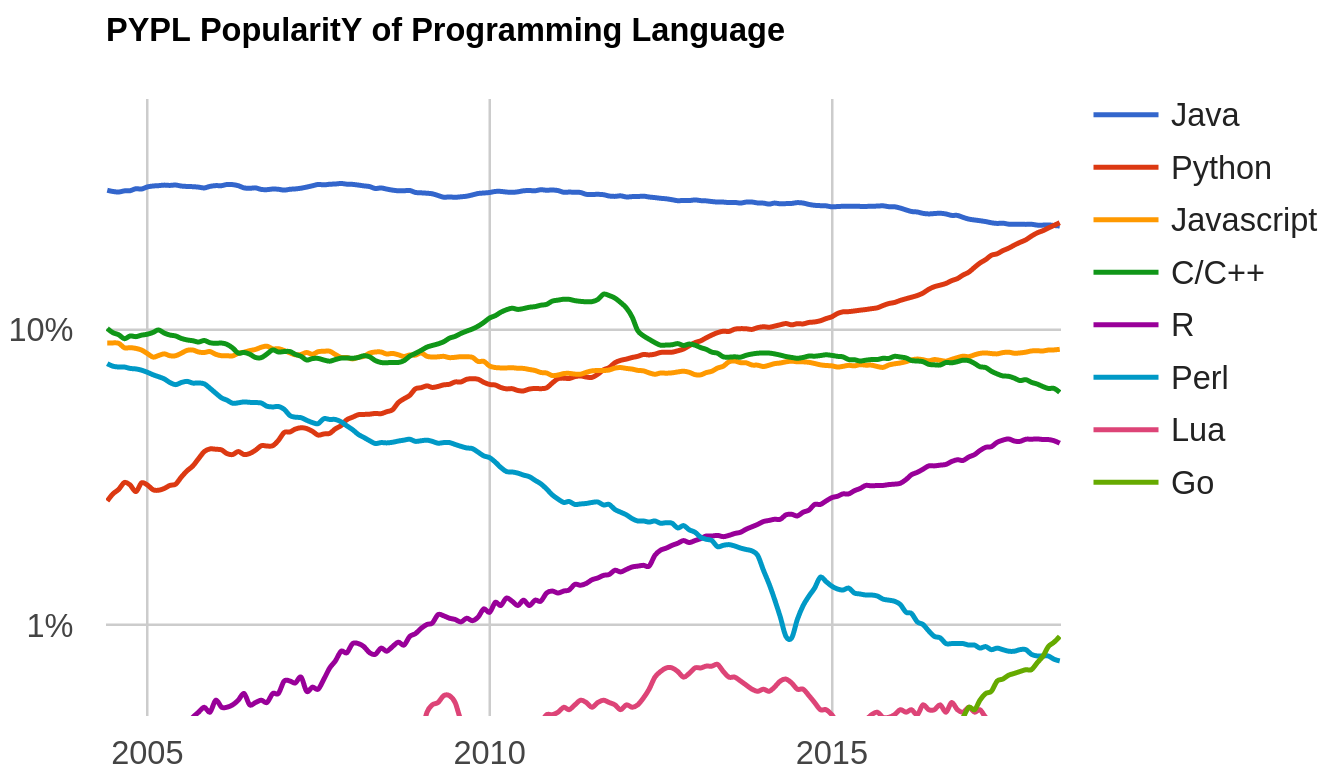
\includegraphics[width=0.8\linewidth]{pypl-popularity.png}
\end{center}
\textcolor{blue}{\scriptsize\url{http://pypl.github.io/PYPL.html}}
\end{frame}

\begin{frame}{In case we need a ``Motivations'' section}
\vspace{0.5 cm}
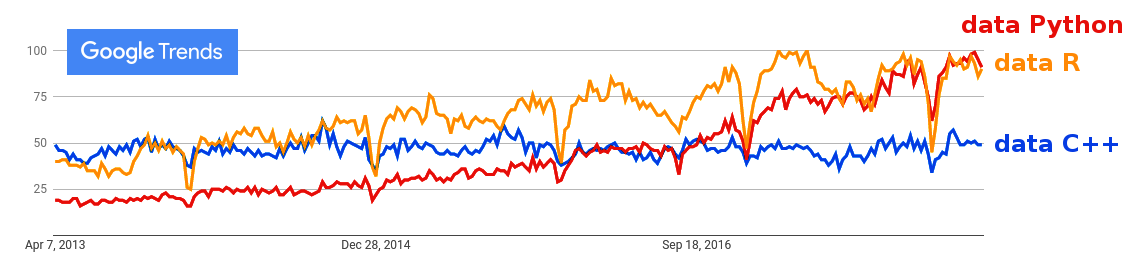
\includegraphics[width=\linewidth]{python-r-cpp-googletrends-data.png}

\vspace{1 cm}
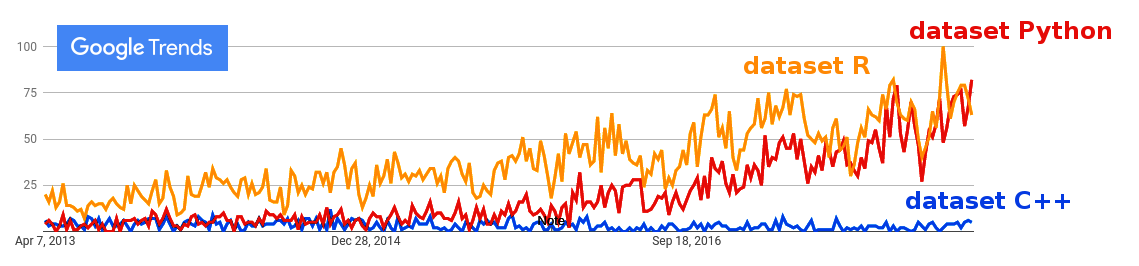
\includegraphics[width=\linewidth]{python-r-cpp-googletrends-dataset.png}
\end{frame}

\begin{frame}{In case we need a ``Motivations'' section}
\vspace{0.5 cm}
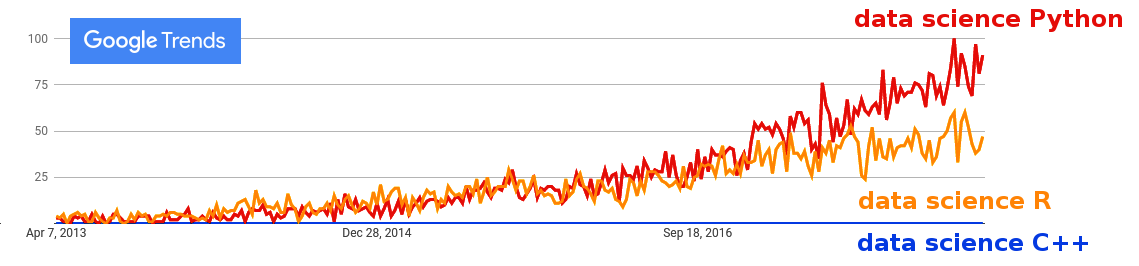
\includegraphics[width=\linewidth]{python-r-cpp-googletrends-datascience.png}

\vspace{1 cm}
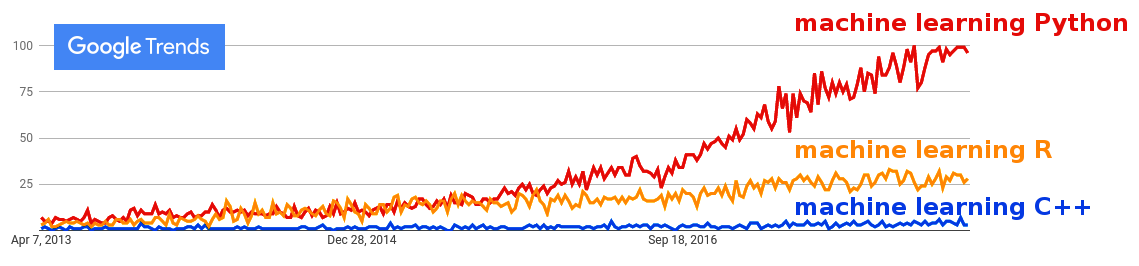
\includegraphics[width=\linewidth]{python-r-cpp-googletrends-machinelearning.png}
\end{frame}

%% \begin{frame}{In case we need a ``Motivations'' section}
%% \vspace{0.5 cm}
%% 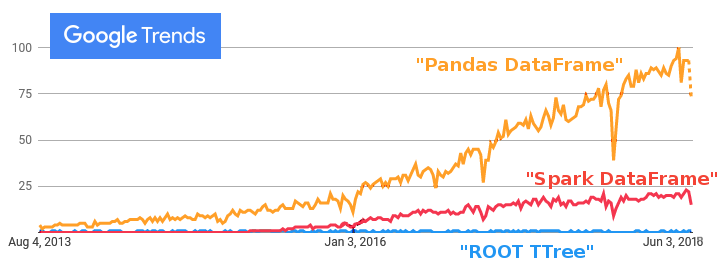
\includegraphics[width=\linewidth]{root-spark-pandas-google-trends.png}
%% \end{frame}

\begin{frame}{Stealing from Jake VanderPlas's {\it Unexpected Effectiveness} talk}
\vspace{0.25 cm}
\begin{columns}[b]
\column{0.75\linewidth}
\only<1>{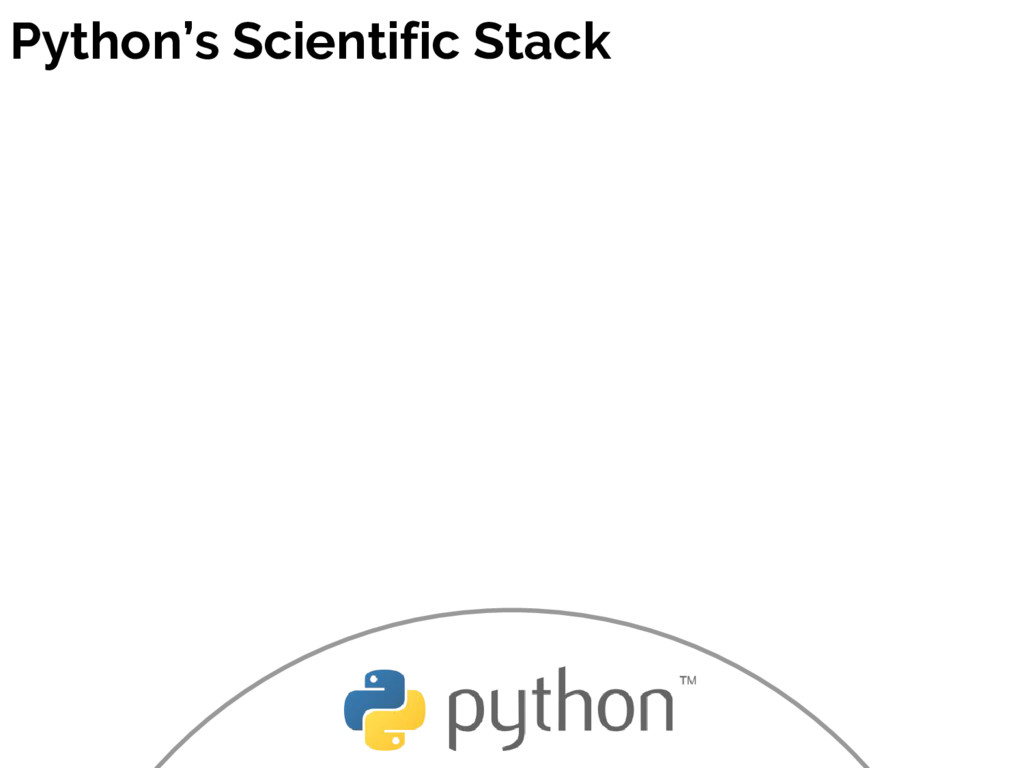
\includegraphics[height=7.8 cm]{shells-1.png}}
\only<2>{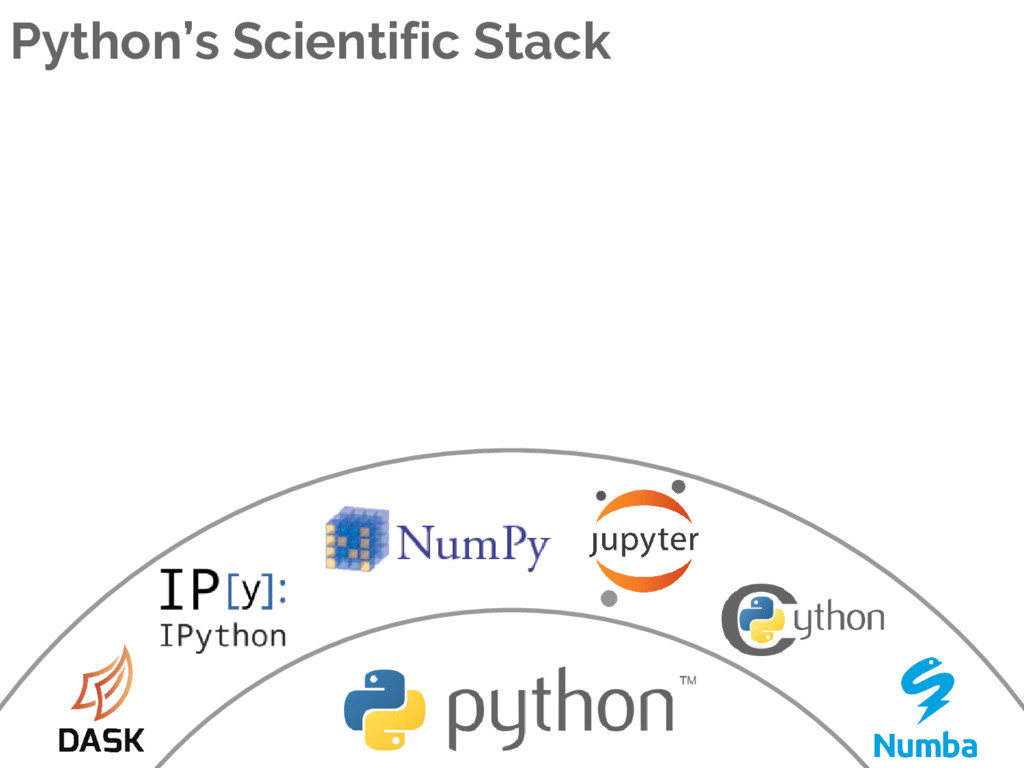
\includegraphics[height=7.8 cm]{shells-2.png}}
\only<3>{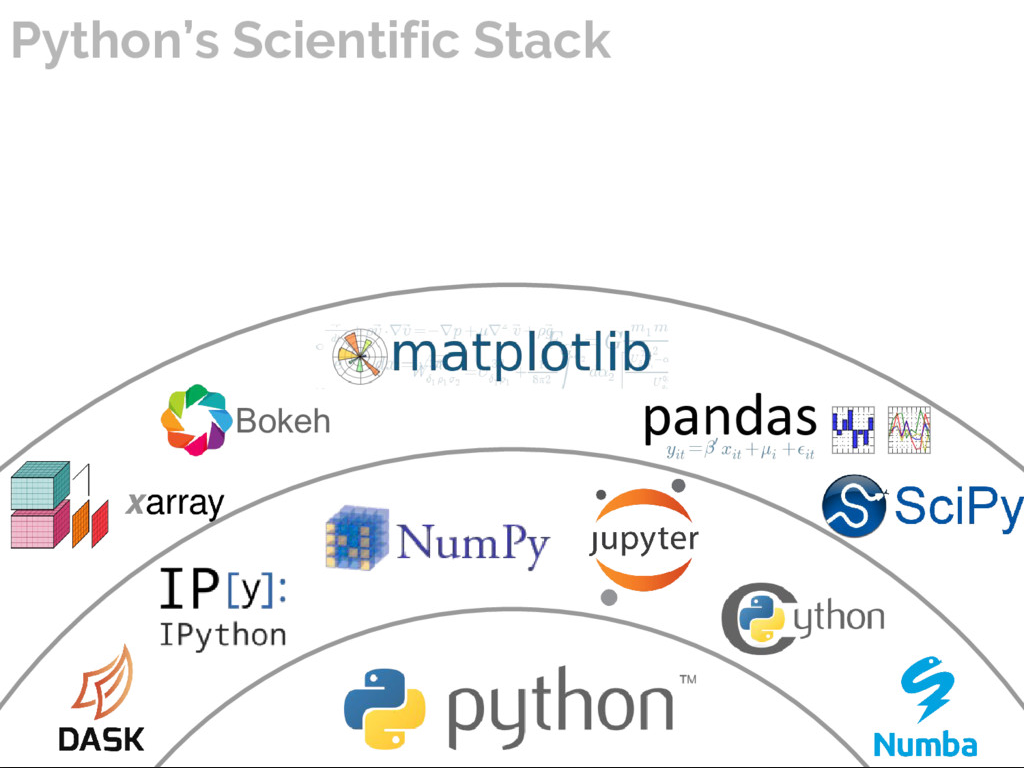
\includegraphics[height=7.8 cm]{shells-3.png}}
\only<4>{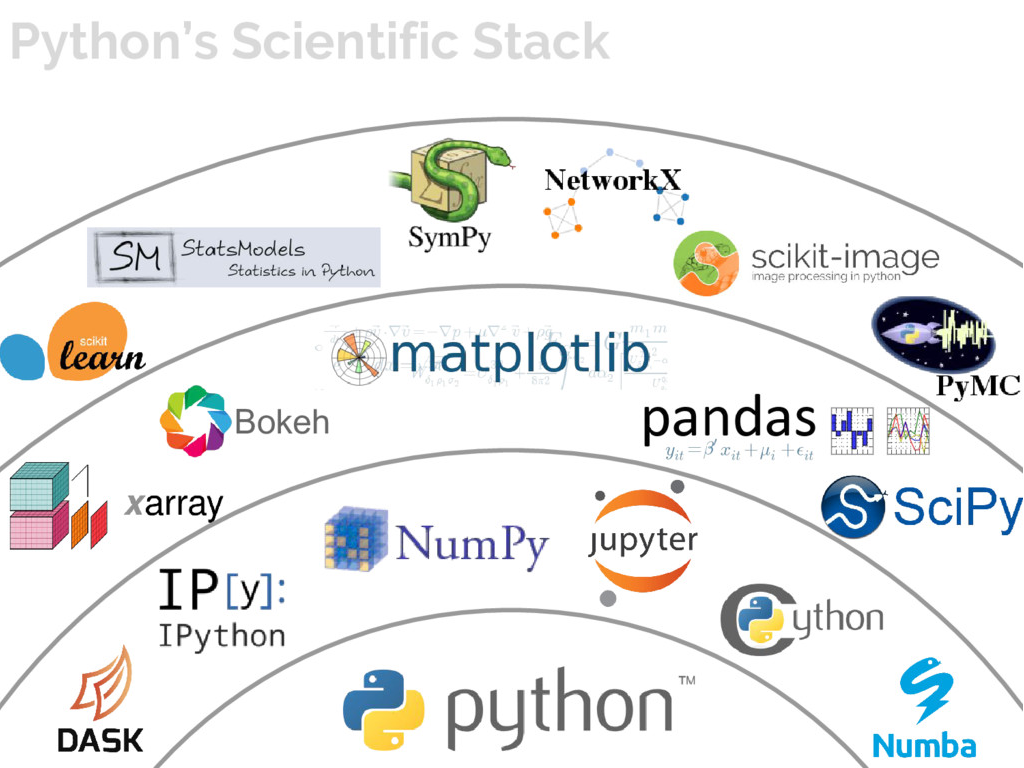
\includegraphics[height=7.8 cm]{shells-4.png}}
\only<5-6>{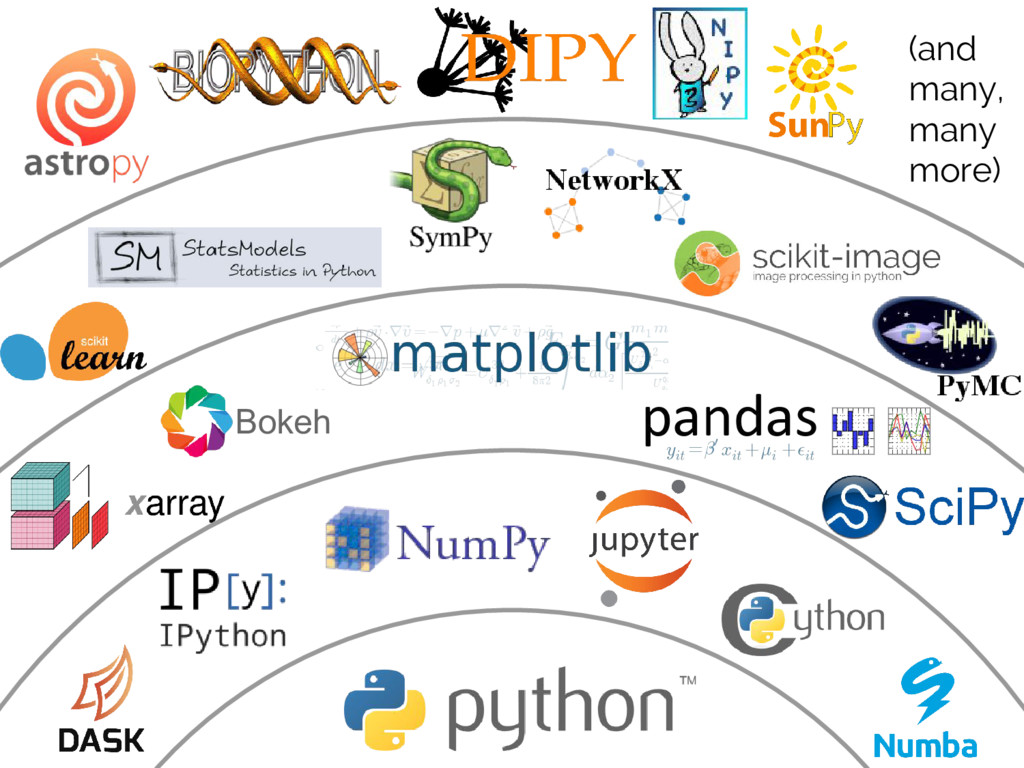
\includegraphics[height=7.8 cm]{shells-5.png}\vspace{0.5 cm}}

\column{0.25\linewidth}

\includegraphics[width=\linewidth]{unreasonable-effectiveness.png}

\vspace{0.5 cm}
\uncover<6>{Searching for packages to do parts of a HEP analysis is eye-opening: you learn what is unique about what we do and what isn't.}

\vspace{-7\baselineskip}
\vspace{4.8 cm}
\end{columns}
\end{frame}

\begin{frame}{The other sciences are doing it, so why can't I?}
\vspace{0.3 cm}
\begin{columns}[b]
\column{0.59\linewidth}
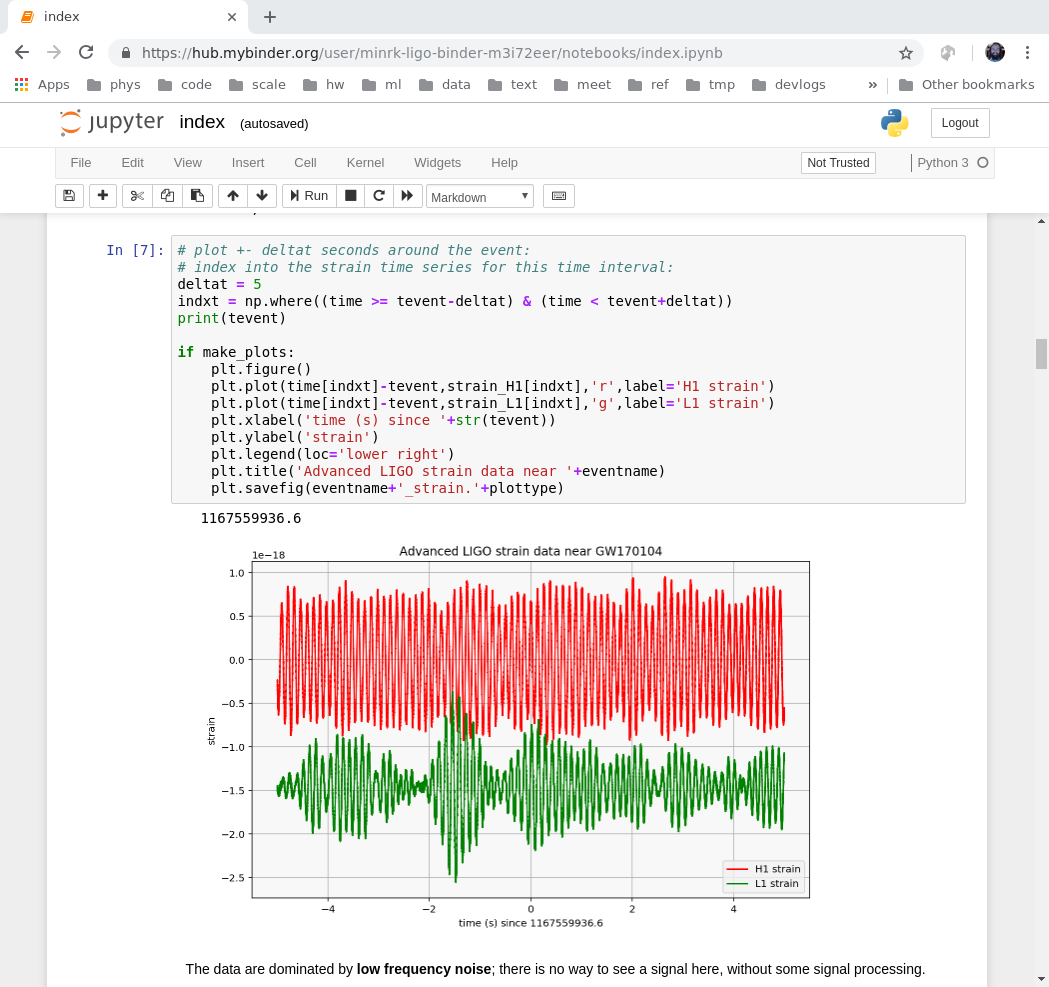
\includegraphics[width=\linewidth]{lsst-notebook.png}

\column{0.41\linewidth}
\begin{itemize}\setlength{\itemsep}{0.5 cm}
\item LIGO full analysis in \\ Numpy $+$ Jupyter $+$ Binder \\ $\to$ you can run all the signal processing yourself without downloading anything.
\item LSST is adopting Python $+$ Jupyter as the general astronomer's interface.
\item XENON-nT is doing their full stack in Python $+$ Numpy.
\item (easy to find examples\ldots)
\end{itemize}

\vspace{0.75 cm}
\end{columns}
\end{frame}

\begin{frame}{Why not indeed?}
\vspace{0.5 cm}
Numpy allowed Python to fill a niche occupied by MATLAB and R: transforming, filtering, signal processing, and machine learning on GB's of rectangular array data.

\vspace{0.75 cm}
\begin{columns}[t]
\column{0.1\linewidth}

\column{0.3\linewidth}
\textcolor{darkgreen}{\bf Python for loops are expressive but not fast.}

\vspace{0.25 cm}
Good for small, complex processing that needs a fully nested object model.

\column{0.3\linewidth}
\textcolor{darkorange}{\bf Numpy arrays are \\ fast but not expressive.}

\vspace{0.25 cm}
Good for biggish, more regular processing (including ML).

\column{0.1\linewidth}
\end{columns}

\vspace{0.75 cm}
Most astronomy, data science, etc.\ fits one of these cases.
\end{frame}

\begin{frame}{Three surmountable challenges}
\large
\vspace{0.5 cm}
\begin{center}
\begin{minipage}{0.75\linewidth}
\begin{enumerate}\setlength{\itemsep}{1 cm}
\item HEP software stacks and conventions were developed {\it before} the Python/Numpy ecosystem and have to be retrofitted to communicate easily.

\item HEP analysis relies heavily on nested data: each event may have a different number of particles.

\item HEP analysis must be performed on TB of ntuples or PB of centrally produced data with thousands of users hitting the same system/files.
\end{enumerate}
\end{minipage}\mbox{\hspace{1 cm}}
\end{center}
\end{frame}

\begin{frame}{}
\LARGE
\vspace{1 cm}
\begin{center}
\textcolor{darkblue}{1. HEP software $\leftrightarrow$ Numpy}
\end{center}
\end{frame}

\begin{frame}{An active area for a long time and now accelerating}
\vspace{0.5 cm}
\begin{itemize}\setlength{\itemsep}{0.5 cm}
\item The PyROOT project started in 2003, just before release 2.3 of \raisebox{-0.2\height}{
\includegraphics[height=\baselineskip]{old-python-logo.png}}.

Every C++ class/function is accessible in Python, at a performance price.

\item Many small HEP packages address specific access issues:

\vspace{0.05 cm}
\begin{itemize}\setlength{\itemsep}{0.05 cm}
\item PyMinuit: extracted from my HEP analysis and open sourced in 2005
\item iminuit: modern version, used in astronomy
\item rootpy: more ``Pythonic'' interface overlaid on PyROOT
\item root\_numpy: faster bindings compiled into C++
\item {\bf 81} packages matching ``HEP'' in PyPI; {\bf 247} with ``HEP'' and Python in GitHub\ldots
\end{itemize}

\item The ROOT team is actively adding ``Pythonizations'' to PyROOT for a more Pythonic interface and also direct-to-Numpy access.

\vspace{0.1 cm}
\begin{itemize}\setlength{\itemsep}{0.1 cm}
\item {\tt\small ttree.AsMatrix()}: access TTree data in Python as Numpy
\item RDataFrame sources and sinks from and to Numpy arrays and Arrow
\end{itemize}
\end{itemize}
\end{frame}

\begin{frame}{Scikit-HEP}
\large
\vspace{0.2 cm}
\begin{columns}
\column{2.5 cm}
\hfill 
\includegraphics[width=0.8\linewidth]{skhep-logo.pdf}

\column{0.8\linewidth}
{\bf Scikit-HEP:} an attempt to build community around a suite of interoperating Pythonic HEP libraries, like PyData or AstroPy.
\end{columns}

\begin{columns}
\column{2.5 cm}
\hfill 
\includegraphics[width=0.8\linewidth]{uproot-logo.pdf}

\column{0.8\linewidth}
{\bf uproot:} reader and writer of the ROOT file format in Python.
\end{columns}

\vspace{0.1 cm}
\begin{columns}
\column{2.5 cm}

\includegraphics[width=\linewidth]{awkward-logo.pdf}

\column{0.8\linewidth}
{\bf awkward-array:} extensions of array programming idioms to non-rectangular and deeply nested data.
\end{columns}

\vspace{0.3 cm}
\begin{columns}
\column{2.5 cm}
\hfill 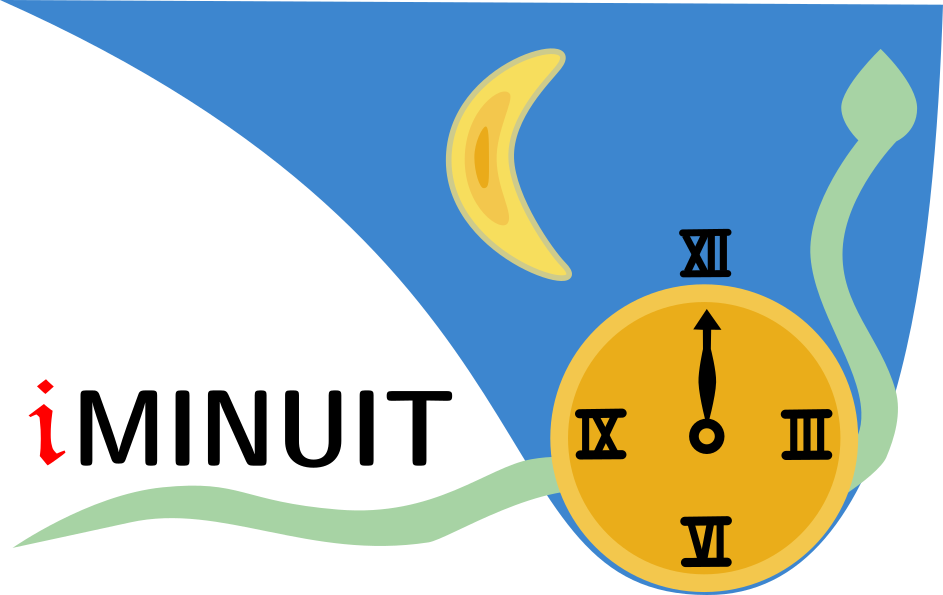
\includegraphics[width=0.8\linewidth]{iminuit-logo.png}

\column{0.8\linewidth}
{\bf iminuit and probfit:} Pythonic interface to Minuit and likelihood builder that works with iminuit.
\end{columns}

\vspace{0.3 cm}
\begin{columns}
\column{2.5 cm}
\column{0.8\linewidth}
{\bf numpythia and pyjet:} interfaces to Pythia and FastJet.
\end{columns}

\vspace{0.3 cm}
\begin{columns}
\column{2.5 cm}
\column{0.8\linewidth}
{\bf decaylanguage, formulate, root\_numpy, vegascope\ldots} packages with focused functionality, broad interfaces.
\end{columns}
\end{frame}

\begin{frame}{uproot}
\hfill \mbox{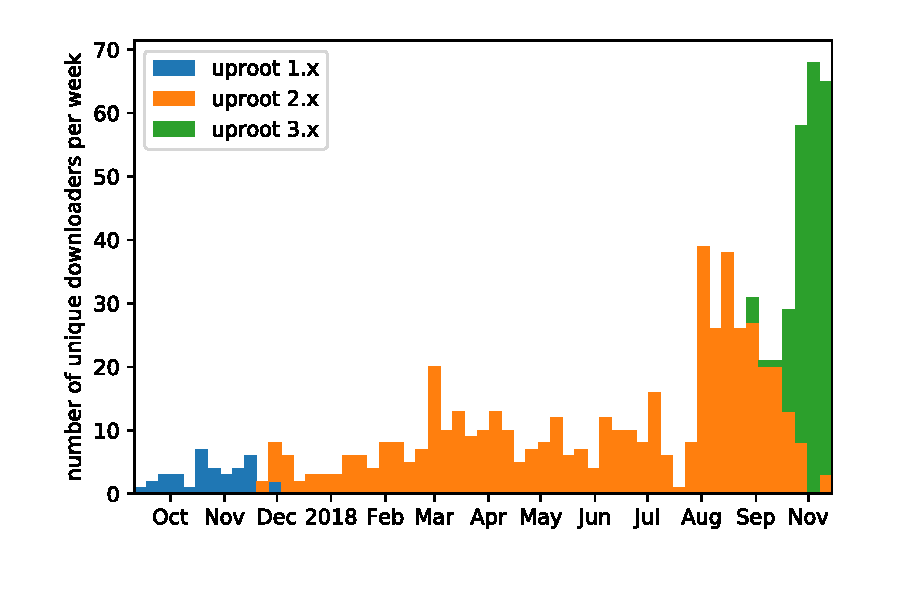
\includegraphics[height=4.5 cm]{weeks_byversion.pdf}\hspace{-1 cm}}

\vspace{-4.25 cm}
Originally, it was a two-week project to access \\ ROOT data in a columnar form more quickly, \\ intended as a backend for a future query service.

\vspace{0.35 cm}
Then I got a lot of feedback from physicists trying \\ to get their data into machine learning libraries.

\vspace{0.35 cm}
So I pivoted, generalized it (2.x), and presented it \\ as an end-user product.

\vspace{0.35 cm}
Most feedback is from users who are trying to do analysis without ROOT:

\vspace{0.05 cm}
\scriptsize
\begin{columns}
\column{0.47\linewidth}
\textcolor{darkgray}{``Great package by the way, the ROOT-independency makes data analysis a lot more flexible.''}

\vspace{0.25 cm}
\textcolor{darkgray}{``Now I'll go through the jagged array tutorial and after that I'll write a wrapper library to make our data accessible without ROOT and any other huge, uncomfortable dependencies, halleluja!''}

\column{0.46\linewidth}

\textcolor{darkgray}{``My particular love of this package is driven by moving away from root as early in my processing as possible and enabling me to use tools I am more comfortable with. I'm not a HEP guy but a space physics guy using geant for instrument responses.''}

\vspace{0.25 cm}
\textcolor{darkgray}{``Thank you for all of your work with this, being able to load root files without ROOT is wonderful!''}
\end{columns}
\end{frame}

%% ``So, in my case, the arrays function are equivalent to numpy load to native format. Very impressive!!! Kudos!!!''

%% ``Also, I'm very excited to see what you do with jagged arrays. They caused me a lot of problems when I started my work with numpy several years ago. I'm happy to know someone is formalizing a way for them to play well with numpy. thanks again for all your work!''

\begin{frame}{uproot implementation philosophy}
\vspace{0.4 cm}
Based on the observation that:
\begin{itemize}
\item a Numpy analysis operates on one column of data at a time, and
\item data in a ROOT file are already arranged in columns.
\end{itemize}

\vspace{0.25 cm}
Transforming columnar bytes on disk into event records back into columnar arrays is undesirable extra work. Dropping that step makes up for seeking to the positions of the columnar arrays using slow Python, {\it if the arrays (baskets) are large.}

\begin{columns}
\column{0.5\linewidth}
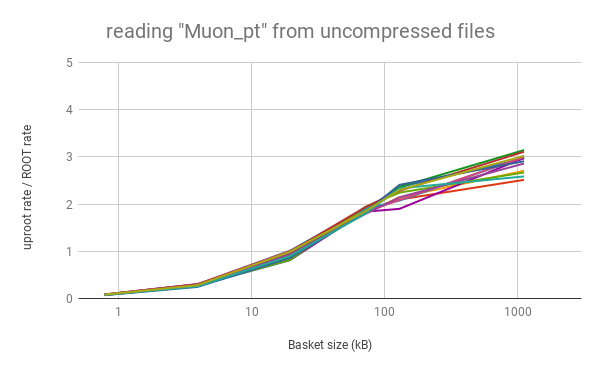
\includegraphics[width=\linewidth]{root-none-muon.png}

\column{0.5\linewidth}
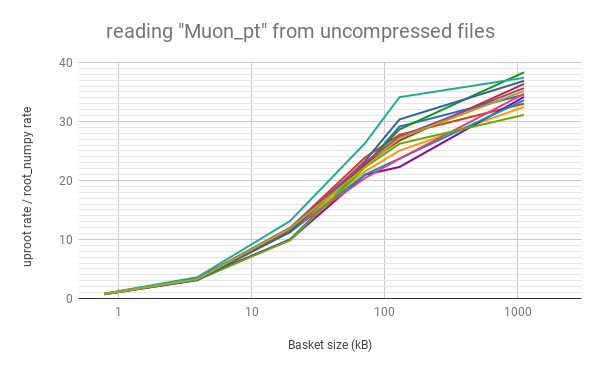
\includegraphics[width=\linewidth]{rootnumpy-none-muon.png}
\end{columns}
\end{frame}

\begin{frame}{uproot dependencies}
\vspace{0.5 cm}
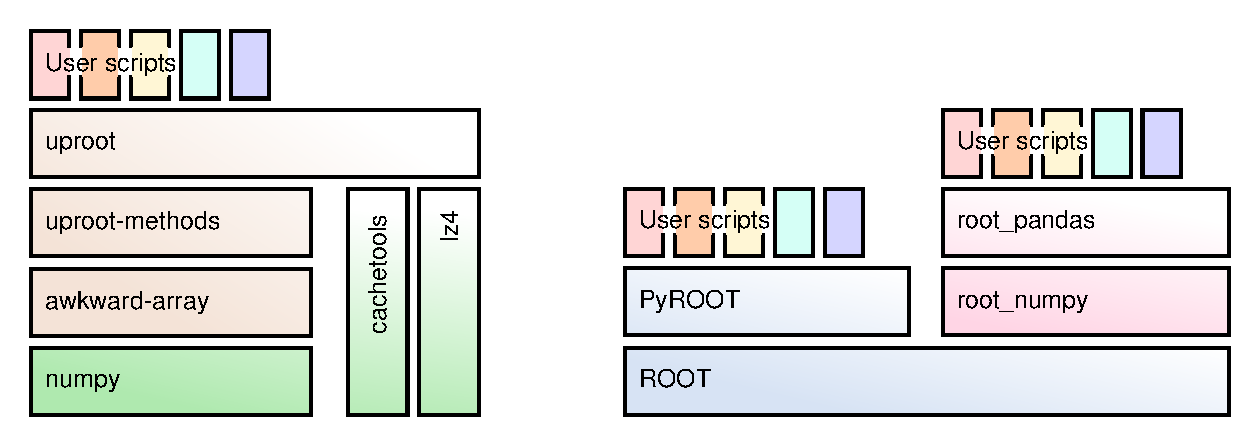
\includegraphics[width=\linewidth]{abstraction-layers.pdf}

\vspace{0.5 cm}
Pythonic interfaces to objects extracted from ROOT (e.g.\ histograms, Lorentz vectors) have been moved to uproot-methods, to evolve on a different schedule and accept more user-contributed pull requests.
\end{frame}

\begin{frame}[fragile]{uproot example: reading and manipulating data}
\small
\vspace{0.1 cm}
\begin{columns}
\column{1.1\linewidth}
\begin{minted}{python}
>>> import uproot
>>> tree = uproot.open("HZZ-objects.root")["events"]   # dict-like
>>> array = tree.array("muonp4")

>>> array                                # all events
<JaggedArray [[TLorentzVector(-52.899, -11.655, -8.1608, 54.779)
               TLorentzVector(37.738, 0.69347, -11.308, 39.402)] ...]>
>>> array[0][1]                          # second particle in first event
TLorentzVector(37.738, 0.69347, -11.308, 39.402)

>>> hastwo = (array.counts >= 2)         # events with at least two muons
>>> leading = array[hastwo, 0]           # mask and select first
>>> subleading = array[hastwo, 1]        # mask and select second

>>> candidates = leading + subleading    # Lorentz vector sum across all
>>> candidates.mass                      # compute mass for all
array([90.22779777, 74.74654928, ..., 85.44384208, 75.96066262])
\end{minted}
\end{columns}
\end{frame}

\begin{frame}[fragile]{uproot example: writing histograms}
\large
\vspace{0.25 cm}
uproot version 3 has write support, but (currently) only for histograms.

\small
\begin{minted}{python}
>>> import uproot
>>> import numpy
>>> file = uproot.recreate("tmp.root")
>>> # give a Numpy histogram a name and save it using file as a dict
>>> file["name"] = numpy.histogram(numpy.random.normal(0, 1, 100000))
\end{minted}

\vspace{1 cm}
\large
Read it back in ROOT:

\small
\begin{minted}{python}
>>> import ROOT
>>> file = ROOT.TFile("tmp.root")
>>> hist = file.Get("name")
>>> hist.Draw()
\end{minted}

\vspace{-3.5 cm}
\hfill 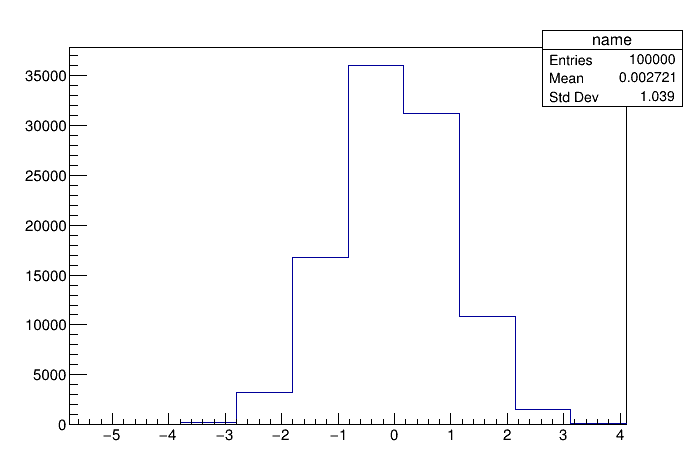
\includegraphics[width=0.5\linewidth]{root-hist.png}
\end{frame}

\begin{frame}{Future directions}
\vspace{0.5 cm}

uproot does its one thing well: just I/O. No major updates forseen for {\it reading,} only bug-fixes and handling corner-case files that users send to me.

\vspace{0.75 cm}
\hfill 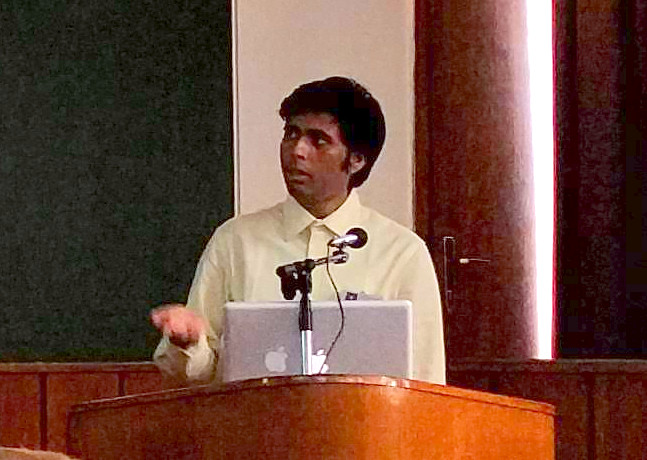
\includegraphics[height=2 cm]{pratyush.jpg}

\vspace{-2 cm}
For {\it writing,} however, I plan to continue to work with Pratyush Das \\ (who added histogram-writing as a DIANA-HEP fellow) to add \\ support for writing simple TTrees on a 6--12~month timescale.

\vspace{0.75 cm}
Small, interacting tools need common protocols. ROOT defines file and C++ protocols; the Scikit-HEP developers are designing in-memory and language-neutral protocols for fit distributions (following SciPy conventions), cost function builders, pseudoexperiments, and histograms (I'm testing Flatbuffers for a wire protocol).
\end{frame}

\begin{frame}{}
\LARGE
\vspace{1 cm}
\begin{center}
\textcolor{darkblue}{2. HEP analysis and nested data structures}
\end{center}
\end{frame}

\begin{frame}{HEP datasets are awkward}
\vspace{0.5 cm}
Most non-HEP data analysis tools (including ML) require rectangular data: a series of equal-sized records. As early as HYDRA and ZBOOK, HEP has required nested data.

\vspace{0.5 cm}
The nested $\to$ tabular transition is lossy! It must be done as late as possible.

\vspace{0.5 cm}
\begin{columns}
\column{0.5\linewidth}
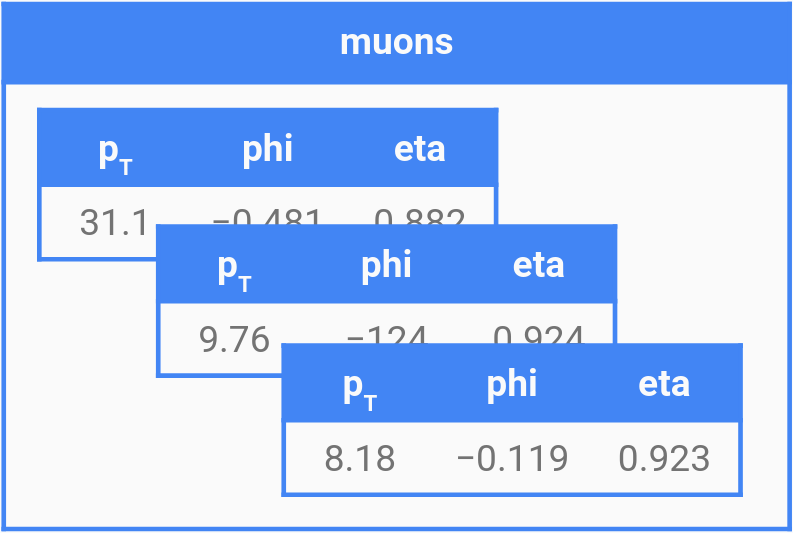
\includegraphics[width=\linewidth]{muons-as-objects.png}

\column{0.5\linewidth}
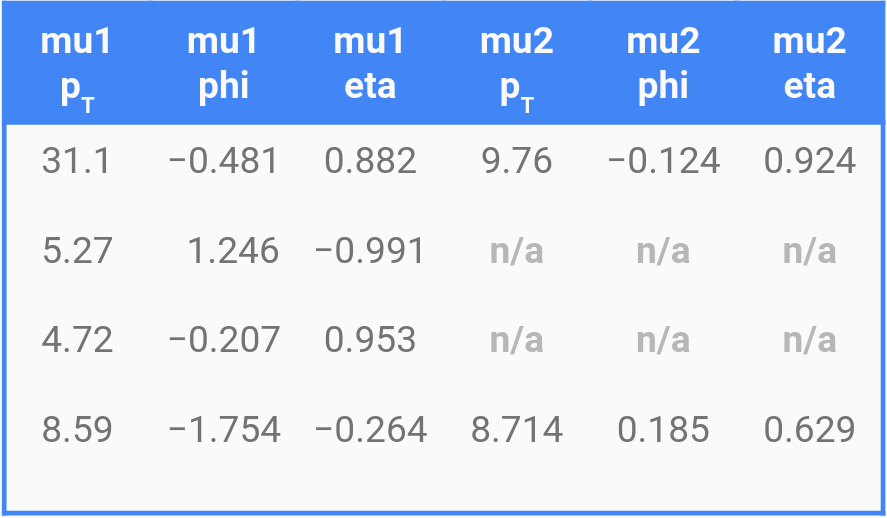
\includegraphics[width=\linewidth]{muons-as-a-table.png}
\end{columns}
\end{frame}

\begin{frame}[fragile]{Jagged arrays}
\vspace{0.5 cm}
uproot required first-order structure just to represent data: jagged arrays.

\vspace{0.5 cm}
Data must appear to be nested lists of variable-length lists but be managed efficiently by arrays. There are several ways to do this and they can be efficiently derived from ROOT files.

\vspace{0.5 cm}
Logical structure: \tabto{3.5 cm}{\ttfamily\textcolor{black}{[\textcolor{red}{[}\textcolor{darkblue}{0, 1, 2}], \textcolor{red}{[}], \textcolor{red}{[}\textcolor{darkblue}{3, 4}], \textcolor{red}{[}\textcolor{darkblue}{5, 6, 7, 8}], \textcolor{red}{[}]\ \ \textcolor{red}{]}}}

\vspace{0.05 cm}
Content:           \tabto{3.5 cm}{\ttfamily\verb|[ |\textcolor{darkblue}{0, 1, 2}\verb|,       |\textcolor{darkblue}{3, 4}\verb|,   |\textcolor{darkblue}{5, 6, 7, 8}\verb|]|}

\vspace{0.05 cm}
Offsets:           \tabto{3.5 cm}{\ttfamily\verb|[|\textcolor{red}{0,}\verb|         |\textcolor{red}{3,}\verb|  |\textcolor{red}{3,}\verb|      |\textcolor{red}{5,}\verb|            |\textcolor{red}{10, 10}\verb|]|}

\vspace{0.05 cm}
Parents:           \tabto{3.5 cm}{\ttfamily\verb|[ |\textcolor{darkgreen}{0, 0, 0}\verb|        |\textcolor{purple}{2, 2,}\verb|   |\textcolor{darkorange}{3, 3, 3, 3}\verb|]|}

\vspace{0.5 cm}
Content $+$ offsets is lossless, compact, and efficient for randomly accessing data.

\vspace{0.1 cm}
Content $+$ parents $+$ total length is lossless, and it makes reduction operations fast.

\vspace{0.1 cm}
Jagged arrays and other primitives can be composed to make any data structure.
\end{frame}

\begin{frame}[fragile]{Array programming: paradigm like object oriented, functional, etc.}
\vspace{0.15 cm}
\hfill 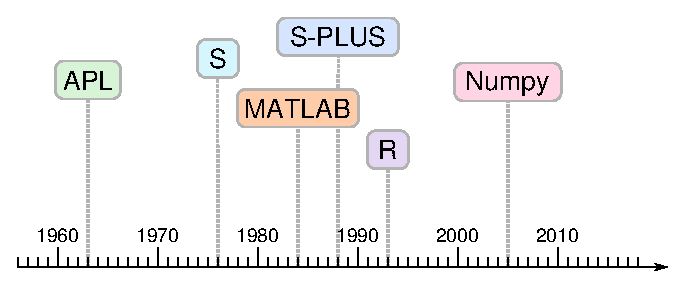
\includegraphics[height=2.75 cm]{apl-timeline.pdf}

\vspace{-2.15 cm}
{\bf\large Array programming: Matlab/R/Numpy}

\vspace{0.5 cm}
Expresses regular operations over \\ rectangular data structures in shorthand.

\vspace{0.25 cm}
\begin{itemize}\setlength{\itemsep}{0.15 cm}
\item Multidimensional slices: \tabto{5.5 cm}{\small \mintinline{python}{rgb_pixels[0, 50:100, ::3]}}
\item Elementwise operations: \tabto{5.5 cm}{\small \mintinline{python}{all_pz = all_pt * sinh(all_eta)}}
\item Broadcasting: \tabto{5.5 cm}{\small \mintinline{python}{all_phi - 2*pi}}
\item Masking (list compaction): \tabto{5.5 cm}{\small \mintinline{python}{data[trigger & (pt > 40)]}}
\item Fancy indexing (gather/scatter): \tabto{5.5 cm}{\small \mintinline{python}{all_eta[argsort(all_pt)]}}
\item Row/column commutativity \tabto{5.5 cm}{\small \mintinline{python}{table["column"][7]} (row 7 of column array)}

(hides AoS $\leftrightarrow$ SoA): \tabto{5.5 cm}{\small \mintinline{python}{table[7]["column"]} (field of row tuple 7)}
\item Array reduction: \tabto{5.5 cm}{\small \mintinline{python}{array.sum()}} $\to$ scalar
\end{itemize}
\end{frame}

\begin{frame}{Extension of array programming to non-rectangular data}
\vspace{0.1 cm}
\begin{columns}
\column{1.05\linewidth}
\begin{itemize}\setlength{\itemsep}{0.15 cm}
\item Multidimensional slices: \tabto{5.5 cm}{\small \mintinline{python}{events["jets"][:, 0]}} $\to$ first jet per event
\item Elementwise operations: \tabto{5.5 cm}{\small \mintinline{python}{jetpt * sinh(jeteta)}} $\to$ \mbox{keep jagged structure\hspace{-1 cm}}
\item Broadcasting: \tabto{5.5 cm}{\small \mintinline{python}{jetphi - metphi}} $\to$ expand {\small \mintinline{python}{metphi}} from

\tabto{5.5 cm}one-per-event to one-per-jet before operation

\item Masking (list compaction): \tabto{5.5 cm}{\small \mintinline{python}{data[trigger]}} $\to$ drop whole events

\tabto{5.5 cm}{\small \mintinline{python}{data[jetpt > 40]}} $\to$ drop jets from events

\item Fancy indexing (gather/scatter): \tabto{5.5 cm}{\small \mintinline{python}{a = argmax(jetpt)}} $\to$ \mbox{\small \mintinline{python}{[[2], [], [1], [4]]}\hspace{-0.5 cm}}

\tabto{5.5 cm}{\small \mintinline{python}{jeteta[a]}} $\to$ \mbox{\small \mintinline{python}{[[3.6], [], [-1.2], [0.4]]}\hspace{-0.5 cm}}

\item Row/column commutativity \tabto{5.5 cm}{\small \mintinline{python}{events["jets"]["pt"][7, 1]}} \mbox{(all the same)\hspace{-0.5 cm}}

(project jagged tables to \tabto{5.5 cm}{\small \mintinline{python}{events["jets"][7]["pt"][1]}}

jagged arrays before indexing): \tabto{5.5 cm}{\small \mintinline{python}{events[7]["jets"]["pt"][1]}}

\tabto{5.5 cm}{\small \mintinline{python}{events["jets"][7, 1]["pt"]}}

\tabto{5.5 cm}{\small \mintinline{python}{events[7]["jets"][1]["pt"]}}

\item Jagged array reduction: \tabto{5.5 cm}{\small \mintinline{python}{jetpt.max()}} $\to$ array of max jet $p_T$ per event
\end{itemize}
\end{columns}
\end{frame}

\begin{frame}[fragile]{Examples from a recent tutorial}
\scriptsize
\vspace{0.25 cm}
\begin{columns}
\column{1.02\linewidth}
\begin{minted}{python}
>>> import awkward
>>> a = awkward.JaggedArray.fromiter([[   1,     2,    3], [], [    4,    5]])
>>> b = awkward.JaggedArray.fromiter([[  10,    20,   30], [], [   40,   50]])
>>> m = awkward.JaggedArray.fromiter([[True, False, True], [], [False, True]])
>>> flat  = numpy.array([  100,  200,  300])
>>> mflat = numpy.array([False, True, True])
>>> i = awkward.JaggedArray.fromiter([[2, 1], [], [1, 1, 0, 1]])

>>> a + b                                     # Elementwise operations
<JaggedArray [[11 22 33] [] [44 55]] at 7b229f329908>

>>> a + flat                                  # Broadcasting
<JaggedArray [[101 102 103] [] [304 305]] at 7b229f7105c0>

>>> a[m]                                      # Masking by jagged (selects particles)
<JaggedArray [[1 3] [] [5]] at 7b229f3290f0>

>>> a[mflat]                                  # Masking by flat (selects events)
<JaggedArray [[] [4 5]] at 7b229f3295c0>

>>> a[i]                                      # Fancy indexing
<JaggedArray [[3 2] [] [5 5 4 5]] at 7b229f3299b0>

>>> a.sum()                                   # Jagged reduction
array([6, 0, 9])
\end{minted}
\end{columns}
\end{frame}

\begin{frame}[fragile]{We can even solve problems with combinatorics}
\vspace{0.35 cm}
{\normalsize\bf Procedural HEP:} selecting the ``best'' leptoquark candidate

\scriptsize
\begin{minted}{python}
leptoquarks = []
for event in dataset:
    best = None
    for jet in event.jets:
        for lepton in event.leptons:
            if cut(jet, lepton):
                leptoquark = jet + lepton        # Lorentz vector + operator
                if best is None or quality(leptoquark) > quality(best):
                    best = leptoquark
    if best is not None:
        leptoquarks.append(best)
\end{minted}

\vspace{0.5 cm}
{\normalsize\bf Jagged array solution:}

\scriptsize
\begin{minted}{python}
pairs = events["jets"].cross(events["leptons"])  # cross-join within events
goodpairs = pairs[cut(pairs["0"], pairs["1"])]   # into pairs["0"] and ["1"]
candidates = pairs["0"] + pairs["1"]             # Lorentz vector + operator
best = candidates[quality(candidates).argmax()]  # best indexes, then objects
leptoquarks = best.flatten()                     # reduce to flat array
\end{minted}
\end{frame}

\begin{frame}{Array programming has competitive performance}
\vspace{0.25 cm}
It isn't just a crutch for slow Python. Efficiency is from SIMD-like data organization.

\vspace{0.4 cm}
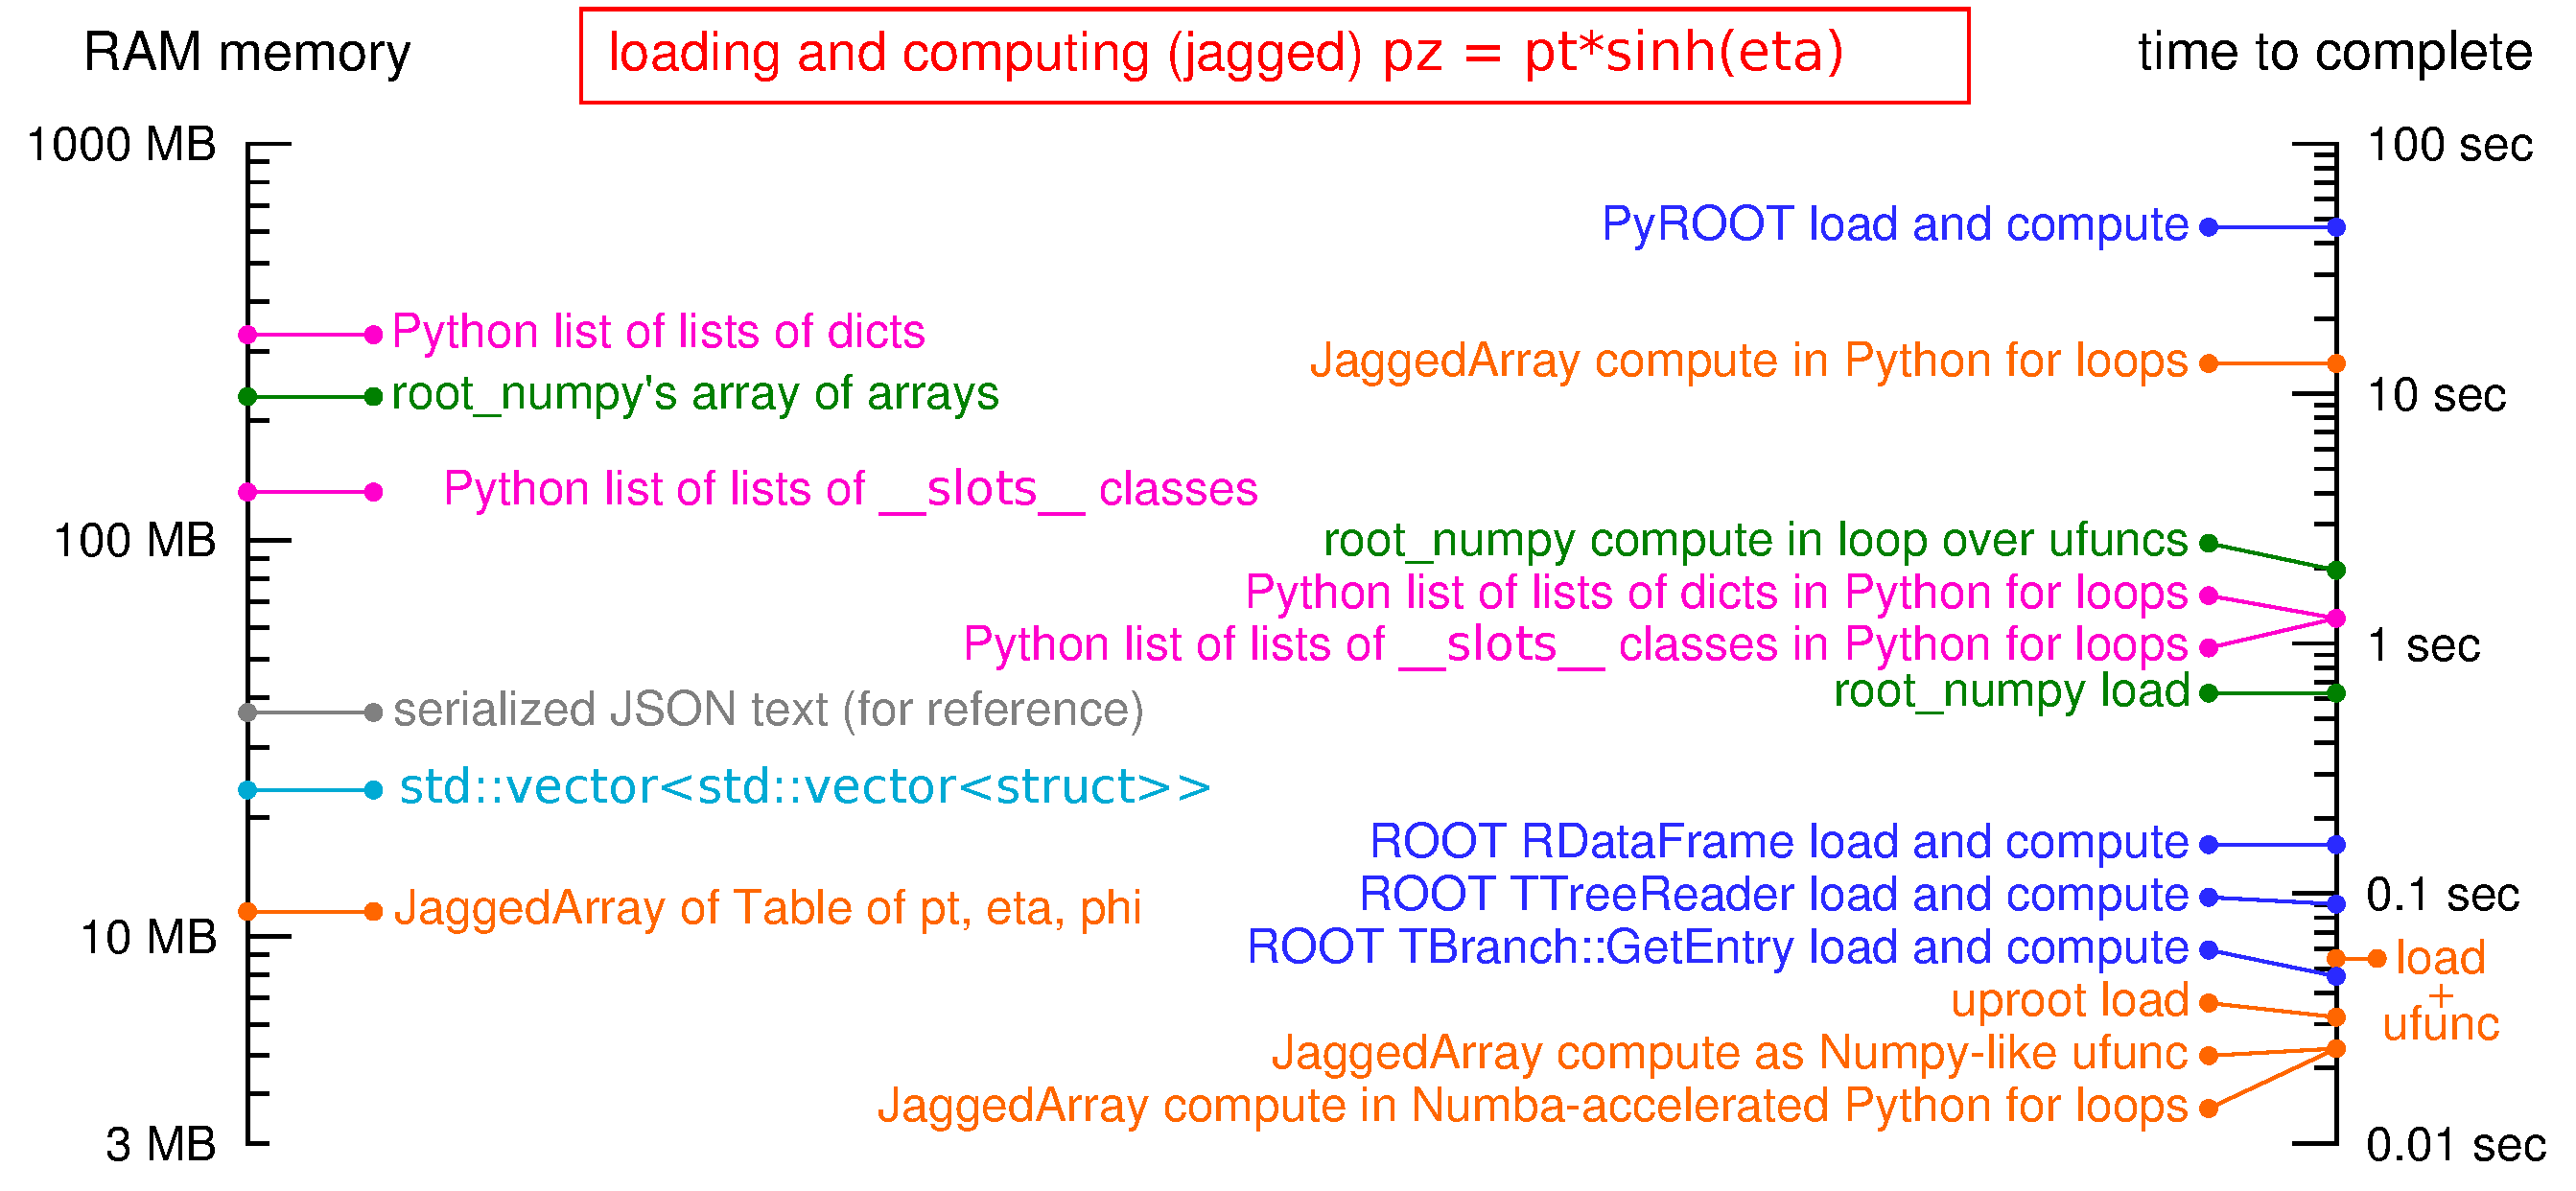
\includegraphics[width=\linewidth]{logscales.pdf}
\end{frame}

\begin{frame}{Once expressed this way, array operations can be highly optimized}
\vspace{0.25 cm}
\hfill 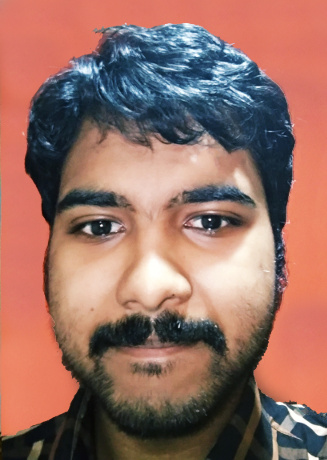
\includegraphics[height=2.5 cm]{jaydeep.jpg}

\vspace{-2.5 cm}
Jaydeep Nandi (GSoC student) developed vectorized implementations of \\ jagged array primitives.

\vspace{0.25 cm}
Below, vectorized-CPU (green) and GPU (red) outperform conventional \\ for-loop versions of {\tt\small jaggedarray.sum()} and {\tt\small jaggedarray.max()}.

\vspace{0.5 cm}
\begin{columns}
\column{0.5\linewidth}
\mbox{ } \hfill Sum of items in groups \hfill \mbox{ }

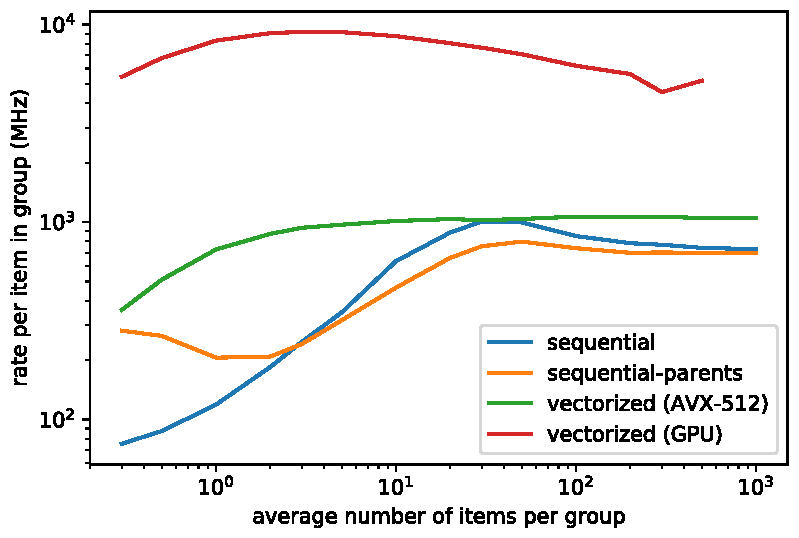
\includegraphics[width=\linewidth]{sum_rates_logy.pdf}

\column{0.5\linewidth}
\mbox{ } \hfill Max of items in groups \hfill \mbox{ }

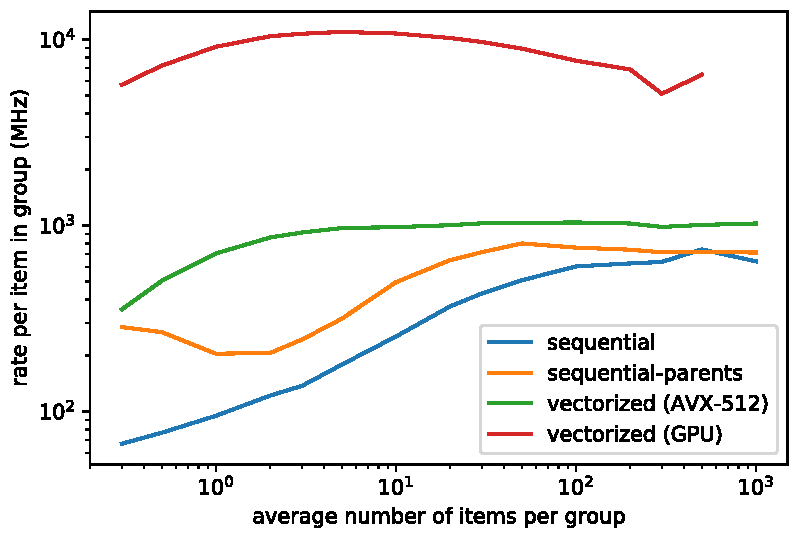
\includegraphics[width=\linewidth]{max_rates_logy.pdf}
\end{columns}
\end{frame}

\begin{frame}{}
\LARGE
\vspace{1 cm}
\begin{center}
\textcolor{darkblue}{3. Scaling up to PB and thousands of users}
\end{center}
\end{frame}

\begin{frame}{Landscape}
\vspace{0.5 cm}
In one way, we don't need anything new: Pythonic array operations can run in a batch job like anything else.

\vspace{0.5 cm}
However, the implicit loop presents an opportunity for transparent multiprocessing: {\tt\small candidates.mass} may be computed for a single particle candidate, an array of millions or a jagged array of billions.

\vspace{0.25 cm}
\begin{itemize}
\item {\bf Dask:} accumulates delayed operations and runs them across all cores or across a cluster of ``thousands.'' Under consideration by LSST.
\item {\bf Joblib:} less fine-grained jobs, dispatching Python functions, not expressions.
\item {\bf Parsl:} also less fine-grained, integrates with traditional schedulers (Condor, Slurm, GRID); academic project from Chicago, Argonne, and Illinois.
\item {\bf PySpark:} if a high-speed bridge from Java to Python (via Arrow) is added.
\end{itemize}

\vspace{0.25 cm}
I'm still hoping we can use off-the-shelf parts; there's a lot still to test.
\end{frame}

\begin{frame}{Future directions}
\large
\vspace{0.5 cm}
Much of my upcoming work involves integrating the awkward-array library with industry tools, to make them more usable in HEP applications:

\begin{center}
\begin{minipage}{0.7\linewidth}
\begin{itemize}
\item {\bf Dask} for distributed processing,
\item {\bf Pandas} for statistics and plotting,
\item {\bf Numba} for JIT-compilation,
\item {\bf blosc/bcolz} for transparent compression,
\item {\bf CuPy} for GPU processing\ldots
\end{itemize}
\end{minipage}
\end{center}

\vspace{0.5 cm}
I've been involved in a half-dozen attempts to scale up analyses with industry tools, some of them just starting. I think we're going to need to try several approaches at the same time.
\end{frame}

\end{document}
